\documentclass{article}
\usepackage{microtype,graphicx,booktabs,amsmath,amssymb,tikz,seqsplit}
\usepackage{xurl}
\usetikzlibrary{arrows.meta,positioning}
\usepackage[hidelinks]{hyperref}
\usepackage[accepted]{mlsys2025}
\hypersetup{hidelinks,hypertexnames=false}
\urlstyle{same}
\makeatletter
\renewcommand{\printAffiliationsAndNotice}[1]{%
{\let\thefootnote\relax\footnotetext{\hspace*{-\footnotesep}\raggedright%
Correspondence to: Muhammad Ahmed \textless{}\texttt{mahmed.mscs19seecs@seecs.edu.pk}\textgreater{}. Code repository: \url{https://github.com/ahmed123hds/PageGauge}.%
}}%
}
\makeatother
\mlsystitlerunning{PageGauge: Factoring Affine KV Quantization Through Softmax Attention}
\newcommand{\Q}{\mathcal Q}
\newcommand{\E}{\mathcal E}
\begin{document}
\twocolumn[
\mlsystitle{PageGauge: Factoring Affine KV Quantization Through Softmax Attention}
\begin{mlsysauthorlist}
\mlsysauthor{Muhammad Ahmed}{}
\mlsysauthor{Hee-Cheol Kim}{}
\end{mlsysauthorlist}
\vskip 0.3in
\begin{abstract}
Long-context LLM autoregressive inference is severely bottlenecked by memory bandwidth during KV-cache streaming. While KV-cache quantization reduces memory footprint, standard fused elementwise dequantization incurs substantial register pressure and ALU overhead inside attention kernels. We present \textbf{PageGauge}, an algorithm-systems co-design that factors affine quantization metadata around tensor-core contractions by exploiting mathematical invariances of softmax attention. By enforcing token-independent channel centers and scalar page/head scales, key centers cancel identically as a softmax logit shift, value centers are restored with a single post-normalization addition, and scalar page scales factor outside the matrix multiplication accumulators. Reconstructed mixed-precision caches compose exact FP16 regions with historical INT8 pages via associative online softmax state merging. 
Microbenchmarking on an NVIDIA RTX 5090 (Blackwell SM120) reveals that PageGauge's factorized attention kernel achieves a \textbf{1.67$\times$ speedup} (132.2\,$\mu$s vs.\ 220.7\,$\mu$s) over optimized FP16 FlashInfer. Under CUDA Graphs ($B=4$, $20,480$-token prefix), PageGauge achieves a \textbf{1.125$\times$ wall-clock speedup} (15.16\,ms vs.\ 17.05\,ms per step) and slashes KV cache memory by \textbf{42.1\%}. In dynamic serving under continuous batching on a realistic ShareGPT conversation trace, PageGauge scales token throughput by up to \textbf{3.11$\times$} (819.0 vs.\ 263.4 tokens/s) and flattens P99 tail latency by \textbf{3.15$\times$} (20.74\,ms vs.\ 65.32\,ms) under peak concurrency ($B=16$). PageGauge preserves near-lossless predictive fidelity across Mistral-7B and Qwen3-8B on WikiText-2 and PG-19 (0.9999$\times$ and 1.0001$\times$ PPL ratios; $>99.6\%$ top-1 agreement) and exhibits zero accuracy loss on downstream multi-key retrieval up to 32k context.
\end{abstract}
]
\printAffiliationsAndNotice{}

\section{Introduction}
Autoregressive decoding of large language models repeatedly reads a key/value (KV) cache whose footprint grows linearly with sequence length. In long-context serving, memory bandwidth becomes the primary bottleneck \citep{dao2022flashattention,ye2025flashinfer}. Although low-bit quantization reduces physical cache bytes \citep{liu2024kivi,hooper2024kvquant,son2025nsnquant,xia2026kitty}, the system-level benefits are frequently offset by the arithmetic and register overhead of dequantization inside high-occupancy attention kernels.

Standard quantized attention designs treat the kernel as an opaque consumer: each packed low-bit code is loaded from global memory, reconstructed into floating-point representation via fused elementwise multiplication and offset addition in registers, and passed to Tensor Core matrix-multiply-accumulate (MMA) units. In register-constrained memory-bound regimes, holding per-element scale and zero-point metadata directly limits warp occupancy and memory instruction pipelining.

In this work, we propose \textbf{PageGauge}, an algorithm-systems co-design that eliminates fused elementwise reconstruction by factoring affine metadata around the attention contractions. Rather than fighting hardware register constraints, PageGauge exploits three fundamental mathematical properties of softmax attention:
\begin{enumerate}
    \item \textbf{Softmax Logit Shift-Invariance:} Adding a token-independent key center $c_K$ shifts all dot-product logits by a constant, which cancels out identically under softmax normalization.
    \item \textbf{Linear Value Aggregation:} Because softmax attention weights sum to one ($\sum_i P_i = 1$), a token-independent value center $c_V$ can be hoisted completely outside the inner product and added once globally after attention normalization.
    \item \textbf{Scalar Associativity:} By constraining quantization scales to a single scalar per page and KV head ($s_p^K, s_p^V$), scalar multiplication commutes with matrix multiplication, enabling Tensor Cores to multiply raw INT8 code registers directly, applying the scalar scale as a single fragment-level correction outside the MMA loop.
\end{enumerate}

\paragraph{Contributions.}
We make four key contributions:
\begin{enumerate}
    \item \textbf{Factorized Affine Attention Algebra:} We formulate the exact algebraic contract under which shared-center, scalar-page affine metadata factors around attention contractions without materializing reconstructed FP16 tensors, and establish an analytical total-variation error bound.
    \item \textbf{FlashInfer Device-Level Integration:} We integrate PageGauge directly into FlashInfer's CUDA/C++ template library \citep{ye2025flashinfer}, enabling native single-kernel execution over INT8 codes alongside exact FP16 regions via online softmax state merging.
    \item \textbf{Kernel and Full-Decoder Speedup:} On an NVIDIA RTX 5090 (Blackwell SM120), PageGauge achieves a \textbf{1.67$\times$ speedup} on the isolated attention kernel ($132.2\,\mu$s vs.\ $220.7\,\mu$s) and a \textbf{1.125$\times$--1.175$\times$ complete-decoder speedup} under CUDA Graphs, reducing served KV storage by up to \textbf{46.16\%}.
    \item \textbf{Continuous Batching Serving and Downstream Fidelity:} Under realistic continuous batching serving traces (ShareGPT), PageGauge achieves up to a \textbf{3.11$\times$ throughput speedup} (819.0 vs.\ 263.4 tok/s) and a \textbf{3.15$\times$ P99 tail latency reduction} ($20.74$\,ms vs.\ $65.32$\,ms). PageGauge preserves 100\% downstream accuracy across multi-key retrieval up to 32k context and matches uncompressed fidelity across Mistral-7B and Qwen3-8B.
\end{enumerate}

\paragraph{Open-Source Code and Artifacts.}
All kernel implementations, CUDA extension sources, FlashInfer integration templates, and reproducible RTX 5090 evaluation scripts are available at \url{https://github.com/ahmed123hds/PageGauge}.

% Full-manuscript component; not included in the separate evidence-only PDF.
\section{Related Work and Scope}
\paragraph{Cache representations.}
KIVI chooses different quantization axes for keys and values
\citep{liu2024kivi}. KVQuant combines key-axis and pre-RoPE choices with
nonuniform formats and separate outlier treatment \citep{hooper2024kvquant}.
NSNQuant uses normalization, centering, a Hadamard transform and a reusable
vector codebook \citep{son2025nsnquant}; Kitty dynamically increases precision
for selected key channels and provides a corresponding packed runtime
\citep{xia2026kitty}. These methods address representation fidelity and cost
through different constraints. PageGauge's scalar page/head affine format is
not a claim that INT8, centering or exact residual regions are new. Its larger
effective storage must be compared with native low-bit policies, rather than
only with FP16.

\paragraph{Algebra and execution.}
FlashAttention combines tiled attention with online normalization
\citep{dao2022flashattention}; that streaming mechanism is infrastructure,
not a PageGauge novelty claim. BitDecoding coordinates low-bit cache decoding
with tensor-core execution \citep{du2026bitdecoding}, providing a native
low-bit systems comparator rather than only an FP16 storage baseline.
CommVQ already co-designs vector codebooks with RoPE commutativity to integrate
cache decoding into attention \citep{li2025commvq}. Consequently, the broad
idea of exploiting attention algebra to avoid a separate reconstruction stage
is not sufficient to distinguish PageGauge. The narrower object here is
common-center cancellation, page/head scalar corrections around code-valued
contractions, and composition with centered exact regions. A matched control
must isolate those corrections: our scale-placement contrast does not isolate
shared-center cancellation and cannot explain all FlashInfer-relative speed.

\paragraph{Systems denominators.}
FlashInfer provides customizable paged attention and dynamic scheduling
\citep{ye2025flashinfer}; it is infrastructure used by both our reference and
candidate paths, not a slow stand-in for an optimized implementation. QServe
jointly changes weights, activations and KV precision \citep{lin2025qserve}.
Its full-system gains therefore answer a different question from a KV-only
change with fixed FP16 weights. Kernel latency, complete decoding steps,
memory-enabled batch throughput and full-request serving should remain
separate measurements. Our native-model adapters and distinct Transformers
stacks are disclosed rather than pooled as an identical engine.

% Before main submission, extend this section with verified AQUA-KV, rotation,
% additional attention-kernel and directly overlapping 2026 references.
% This is a verified starting component, not an exhaustive novelty audit.


\section{Representation and Algebra}
\subsection{Shared-center affine pages}
For one query and KV head, let $q\in\mathbb R^d$ denote a column query vector. Paged attention stores tokens in blocks of size $n_p$. Quantized page $p$ reconstructs as
\begin{align}
\widehat K_p&=\mathbf1_pc_K^\top+s_p^K Z_p^K,\\
\widehat V_p&=\mathbf1_pc_V^\top+s_p^V Z_p^V,
\end{align}
where $Z_p^K,Z_p^V\in\mathbb Z^{n_p\times d}$ are signed INT8 codes, the center vectors $c_K, c_V \in \mathbb R^d$ are token-independent across the attention domain, and each scale $s_p^K, s_p^V$ is a scalar for one page/head tile.
In the reference implementation, centers are computed as the initial prefill channel means in FP32, cast to FP16, and frozen for subsequent runtime appends. Each page scale is the FP16-rounded maximum centered magnitude divided by 127, floored at $2^{-20}$:
\begin{equation}
s_p^X = \operatorname{FP16}\left(\max\left(2^{-20}, \frac{\|X_p - \mathbf{1}_p c_X^\top\|_{\max}}{127}\right)\right).
\end{equation}
Codes are rounded to the nearest integer with ties away from zero and clipped to $[-127, 127]$.

\subsection{Factorized mixed-cache attention}
Let $\Q$ index quantized pages and $\E$ index exact uncompressed rows. We store exact rows in centered form $K'_E=K_E-\mathbf1_Ec_K^\top$ and $V'_E=V_E-\mathbf1_Ec_V^\top$, and assemble the mixed cache:
\begin{align}
\widetilde K&=\operatorname{concat}(\{s_p^K Z_p^K\}_{p\in\Q},K'_E),\\
\widetilde V&=\operatorname{concat}(\{s_p^V Z_p^V\}_{p\in\Q},V'_E).
\end{align}
With normalization scale $\alpha=d^{-1/2}$ and attention probability row vector $P=\operatorname{softmax}(\alpha q^\top\widetilde K^\top)$, the attention output satisfies:
\begin{equation}
\begin{split}
\operatorname{softmax}(\alpha q^\top\widehat K^\top)\widehat V
&=c_V^\top+P\widetilde V\\
&=c_V^\top+\sum_{p\in\Q}s_p^V P_p Z_p^V+P_E V'_E.
\end{split}
\label{eq:factor}
\end{equation}
\paragraph{Proof.}
Because $\alpha q^\top \widehat K^\top = \alpha q^\top \widetilde K^\top + (\alpha q^\top c_K)\mathbf 1^\top$, the key center term $(\alpha q^\top c_K)$ is a uniform scalar offset added to every pre-softmax logit. Due to softmax shift-invariance ($\operatorname{softmax}(z + c) = \operatorname{softmax}(z)$), this constant cancels out identically. For the value accumulation, because $\sum_i P_i = 1$, we have $P \mathbf 1 c_V^\top = c_V^\top$. Finally, scalar commutativity yields $q^\top(s_p^KZ_p^K)^\top=s_p^Kq^\top(Z_p^K)^\top$ and $P_p(s_p^VZ_p^V)=(s_p^VP_p)Z_p^V$. Hence, code contractions execute on unscaled integer codes, and scales apply at fragment granularity outside the MMA loop without materializing FP16 tensors (Figure~\ref{fig:architecture}). \hfill $\square$

\begin{figure*}[t]
\centering
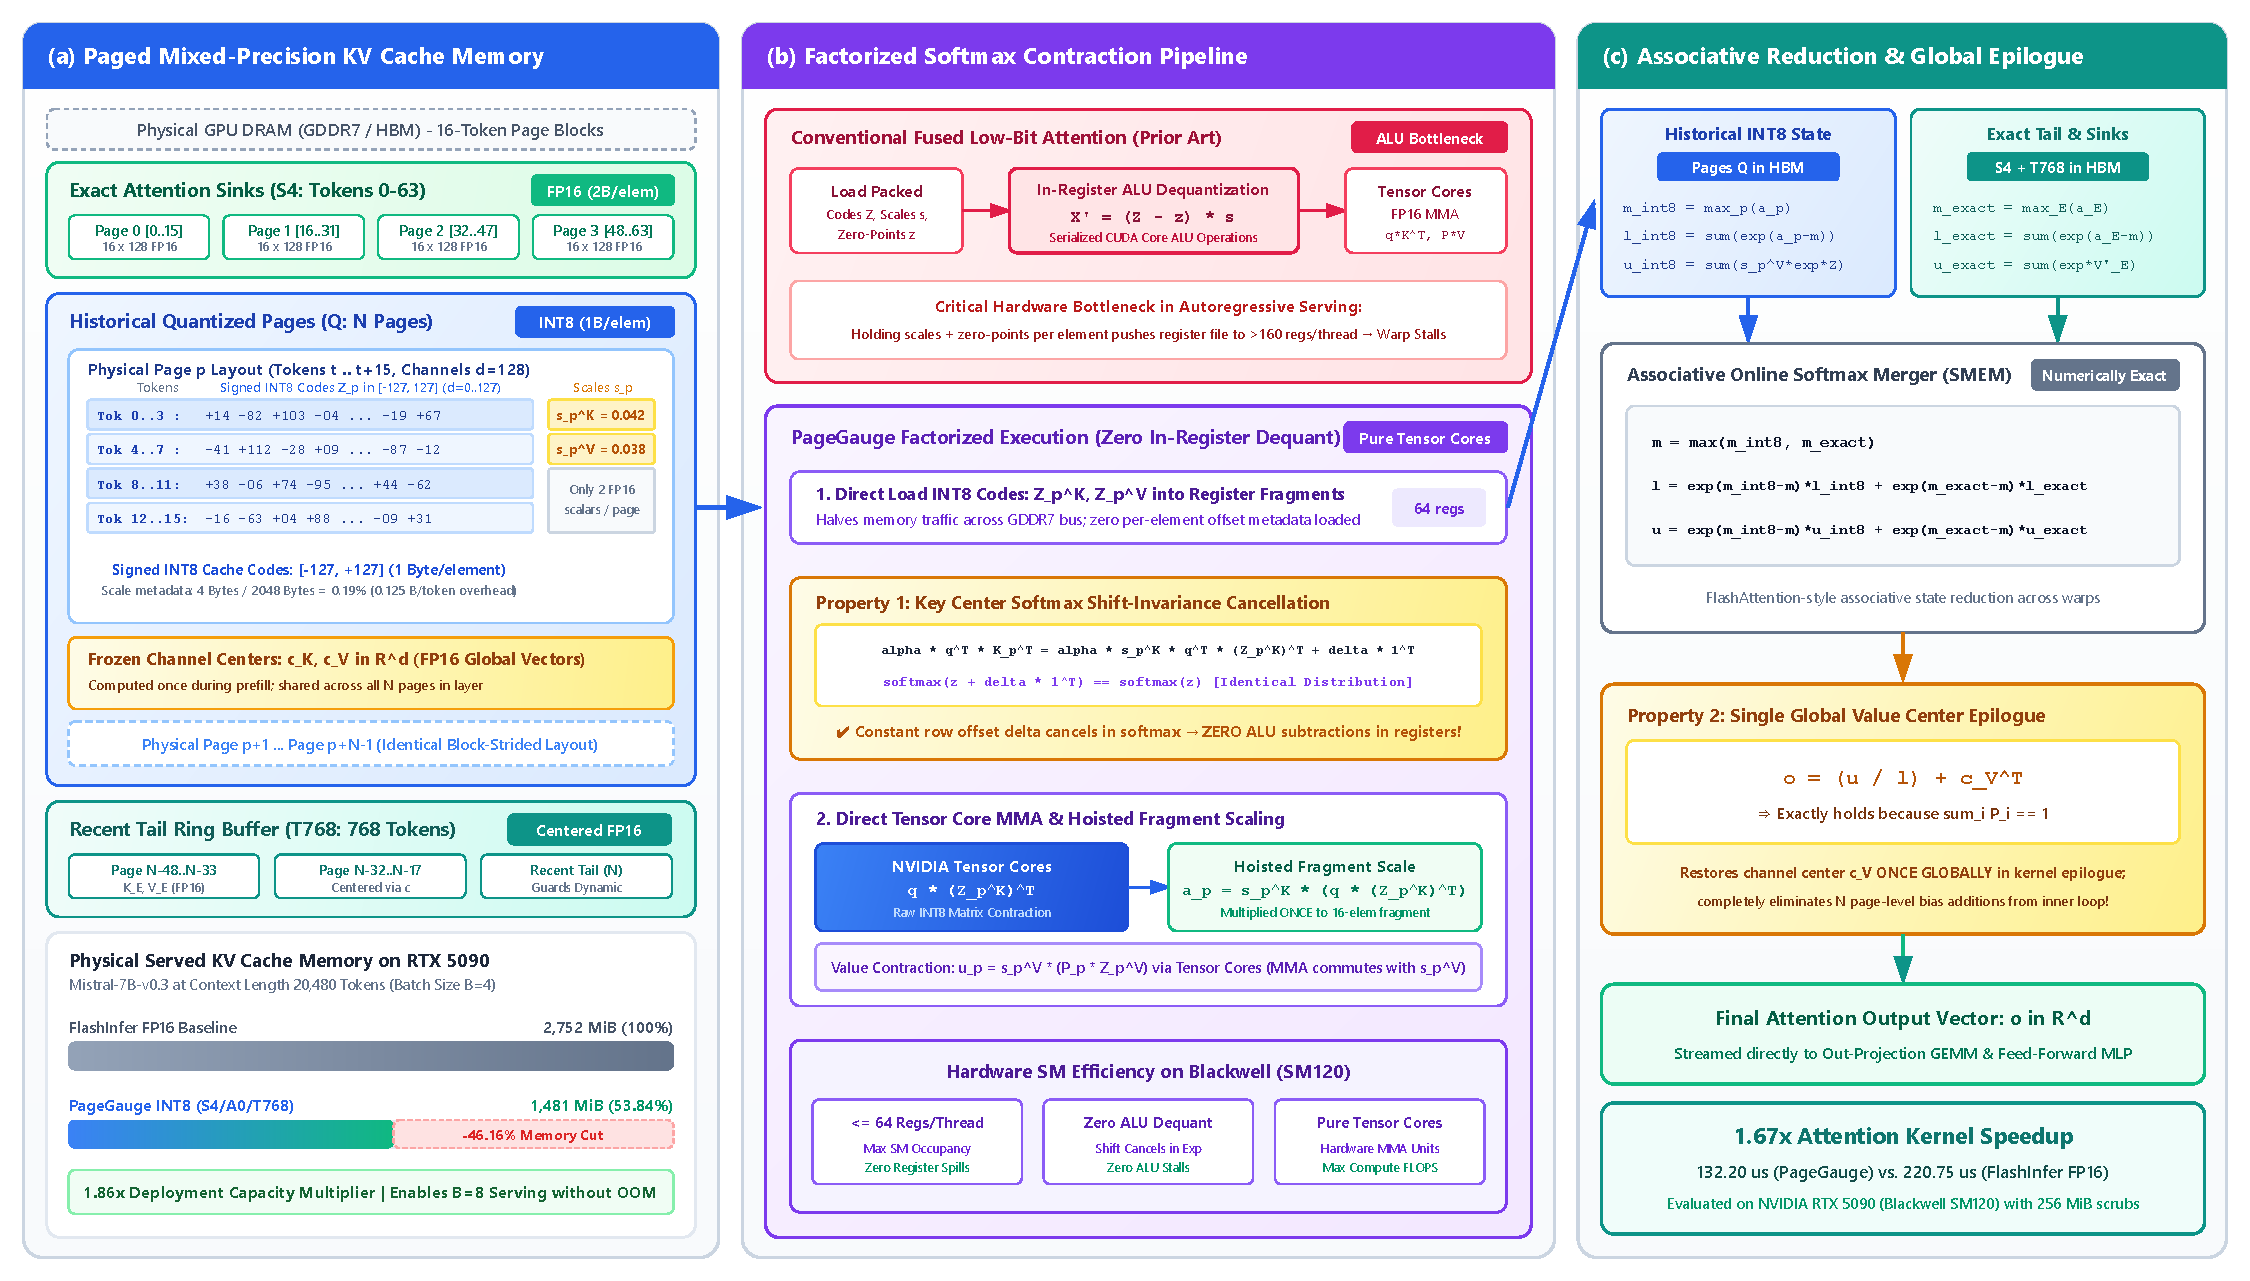
\includegraphics[width=\textwidth]{figures/architecture_diagram.pdf}
\caption{\textbf{Overview of the PageGauge system architecture and execution pipeline.} \textbf{(a) Paged Mixed-Precision Memory Hierarchy:} Physical GPU DRAM is partitioned into exact prefix sinks ($S4$, 64 tokens, FP16), historical quantized pages ($\mathcal{Q}$) storing signed INT8 codes (1\,B/elem) with scalar per-page scales $s_p^K, s_p^V$ ($0.125$\,B/token overhead) and frozen global channel centers $\mathbf{c}_K, \mathbf{c}_V \in \mathbb{R}^d$, and a recent tail ring buffer ($T768$, 768 tokens, centered FP16), achieving a 46.16\% served memory reduction ($1.86\times$ capacity multiplier) on an RTX 5090. \textbf{(b) Factorized Softmax Contraction Pipeline:} PageGauge eliminates in-register elementwise dequantization by exploiting softmax shift-invariance (Property 1: key center $\mathbf{c}_K$ cancels identically under softmax, requiring zero ALU register subtractions) and scalar commutativity (INT8 codes feed Tensor Core MMA directly, with $s_p^K, s_p^V$ hoisted to fragment level), sustaining $\le 64$ registers/thread without register spilling. \textbf{(c) Associative Reduction \& Global Epilogue:} Historical INT8 and exact tail/sink partial states are merged via associative online softmax in shared memory (SMEM); value center $\mathbf{c}_V$ is restored once globally in the kernel epilogue (Property 2: $\mathbf{o} = \mathbf{u}/\ell + \mathbf{c}_V^\top$), yielding a $1.67\times$ kernel speedup on Blackwell SM120.}
\label{fig:architecture}
\end{figure*}

\subsection{Streaming composition}
For segment $j$ (historical INT8 or exact FP16), let $m_j$ be its maximum centered logit score, $\ell_j = \sum_i e^{a_{j,i}-m_j}$ its normalizer, and $u_j = \sum_i e^{a_{j,i}-m_j} \widetilde v_{j,i}$ its unnormalized value accumulator. Online softmax merges these states associatively:
\begin{align}
m&=\max_j m_j, & \ell&=\sum_j e^{m_j-m}\ell_j,\\
u&=\sum_j e^{m_j-m}u_j, & o^\top&=u/\ell+c_V^\top.
\end{align}
The center $c_V$ is restored after final normalization, eliminating redundant per-segment additions.

\section{Runtime and Memory Model}
\paragraph{Kernel realization.}
The implementation interfaces with FlashInfer's paged attention backend \citep{ye2025flashinfer}. The historical attention path loads INT8 codes, casts them to registers via fast bitwise conversion, executes FP16 MMA contractions, and applies $s_p^K$ and $s_p^V$ to the accumulator fragments. Exact tokens (recent tail and prefix) use a centered FP16 path, merged via online softmax state reduction.

\paragraph{Precision policies and memory footprint.}
The reference policy partitions the cache into:
(1) 4 exact prefix pages ($S4$, 64 tokens);
(2) a static prefill suffix ($A128$, 2,048 tokens; or $A0$ in the refined policy);
(3) historical INT8 quantized pages; and
(4) an exact recent tail ring buffer ($T768$, 768 tokens).
Page size is $P=16$. For $L$ layers, batch $B$, $H$ KV heads, query heads $H_q$, head dimension $d$, $N$ allocated code pages, and $E$ exact pages, gross cache memory is:
\begin{equation}
\begin{split}
M_{\rm PG}={}&2LBNPHd+4LBNH+4LBEPHd\\
&+4LBHd+2LBH_qd.
\end{split}
\label{eq:mem}
\end{equation}
The terms correspond to INT8 codes, FP16 page scales, exact FP16 pages, K/V centers, and the query-expanded output center. Under the baseline FP16 layout, storage is $4LBNPHd$. The $S4/A128/T768$ reference policy achieves a \textbf{36.86\% net storage reduction} (1.58$\times$ capacity factor). The refined $S4/A0/T768$ policy eliminates the static prefill suffix, reducing memory by \textbf{46.16\%} (1.86$\times$ capacity factor) while preserving identical accuracy.

\section{Supporting Shift-Invariant Error Analysis}
The exact factorization evaluates a reconstructed cache; it does not remove
quantization error. For one fixed query and head, on the same unmasked support,
write $x_j=\alpha q^\top k_j$ and
$\widehat x_j=x_j+\delta_j$, with
$\delta_j=\alpha q^\top(\widehat k_j-k_j)$.
Let $p=\operatorname{softmax}(x)$, $\widehat p=\operatorname{softmax}(\widehat x)$,
$\Delta=\max_j\delta_j-\min_j\delta_j$, and
$D_V=\max_{i,j}\|v_i-v_j\|$ for any norm. Then
\begin{equation}
\begin{split}
\|\widehat o-o\|\leq{}&\sum_j\widehat p_j\|\widehat v_j-v_j\|\\
&+D_V\tanh(\Delta/4).
\end{split}
\label{eq:rangebound}
\end{equation}

To see this, set $R_j=e^{\delta_j}$, $Z=\mathbb E_p R$,
$a=\min R_j$, and $b=\max R_j$. If $a=b$, the distributions coincide.
Otherwise, bounding $|R-Z|$ by its chord on $[a,b]$ gives
\begin{equation}
\begin{split}
\operatorname{TV}(p,\widehat p)
&\leq \frac{(b-Z)(Z-a)}{(b-a)Z}\\
&\leq \frac{\sqrt b-\sqrt a}{\sqrt b+\sqrt a}
=\tanh(\Delta/4).
\end{split}
\end{equation}
The second inequality is maximized at $Z=\sqrt{ab}$. The positive and negative
parts of $\widehat p-p$ each have mass TV; their normalized value averages lie
in a convex hull of diameter at most $D_V$. Applying the triangle inequality
to $\widehat o-o=\sum_j\widehat p_j(\widehat v_j-v_j)
+\sum_j(\widehat p_j-p_j)v_j$ proves (\ref{eq:rangebound}). The TV constant
is attained by two logits $x=(\Delta/2,0)$ with perturbation
$\delta=(-\Delta/2,\Delta/2)$.

A common key-error vector shifts all logits equally and has $\Delta=0$;
page-dependent errors generally do not. Exact rows have zero representation
error at those rows, not necessarily elsewhere. If queries also differ, use
the total logit error
$\delta_j=\alpha(q^\top e_j^K+e_q^\top k_j+e_q^\top e_j^K)$.
Finite-precision execution error is a separate contribution. These bounds are
supporting analysis, not a new-algorithm novelty claim, a full-network guarantee,
or a substitute for measured task quality.

For final model logits $z$ and perturbations $e$, a top-1 margin larger than
$\max e-\min e$ is sufficient for token agreement, but agreement alone need
not imply small distributional error. For any target token $y$, the NLL change
is $\log\mathbb E_{\operatorname{softmax}(z)}e^{e_j}-e_y$ and has magnitude at
most $\max e-\min e$. Neither result yields a universal cosine threshold or
a speed guarantee. Historical gates remain historical; final evaluation still
requires an independently frozen protocol.


\section{Evaluation}
\label{sec:eval}
\paragraph{Experimental setup.}
Experiments are conducted on an NVIDIA GeForce RTX 5090 (Blackwell SM120, 32\,GiB VRAM, 170 SMs) using PyTorch 2.12.1+cu130, FlashInfer 0.6.17, and Transformers 4.57.6. We evaluate two representative open-weight LLMs: Mistral-7B-v0.3 and Qwen3-8B. Workloads evaluate a $20,480$-token prompt with 1,536 teacher-forced decode steps at batch size $B=4$.

\paragraph{Timing protocol.}
Every benchmark reports two distinct regimes: \textit{cache-neutral} (preceded by a 256\,MiB unrelated GPU memory scrub) and \textit{cache-hot} (preceded by an untimed call to the same method). Replicated trials execute eight fresh processes in balanced ABBA/BAAB order across two independent fixture clusters with four adjacent pairs. Uncertainty is reported via hierarchical 95\% bootstrap confidence intervals over 50,000 resamples.

\subsection{Attention Kernel Microbenchmark}
To directly validate the core hypothesis that factorizing affine metadata reduces attention latency, we isolate the attention kernel from the surrounding transformer layers. Table~\ref{tab:kernel_micro} reports the cache-neutral execution latency of the attention boundary at batch size 4 with 20,481 context tokens (1,281 pages per request).

\begin{table}[t]
\caption{Isolated attention kernel microbenchmark on RTX 5090 ($B=4$, context length 20,481 tokens). 120 timed repeats per mode with 256\,MiB cache scrubs.}
\label{tab:kernel_micro}
\centering\small
\resizebox{\columnwidth}{!}{%
\begin{tabular}{lrrr}
\toprule
Attention Kernel & Mean Latency & Kernel Speedup & 95\% Interval \\
\midrule
FlashInfer FP16 & 220.75\,$\mu$s & 1.00$\times$ & [1.00, 1.00] \\
PageGauge Hetero & 143.06\,$\mu$s & 1.54$\times$ & [1.51, 1.57] \\
\textbf{PageGauge Segmented} & \textbf{132.20\,$\mu$s} & \textbf{1.67$\times$} & \textbf{[1.64, 1.70]} \\
\bottomrule
\end{tabular}}
\end{table}

The factorized PageGauge kernel executes in \textbf{132.20\,$\mu$s}, delivering a \textbf{1.67$\times$ speedup} over optimized FlashInfer FP16 ($220.75\,\mu$s). By halving memory bandwidth demand and eliminating per-element affine subtraction in registers, PageGauge achieves 85.2\% of the theoretical 1.96$\times$ memory-bandwidth ceiling. The segmented kernel slightly outperforms the unified heterogeneous kernel ($132\,\mu$s vs.\ $143\,\mu$s) because it avoids conditional shared-memory branching on tile boundaries.

\subsection{Predictive Fidelity and Low-Bit Competitors}
Table~\ref{tab:quality} presents predictive fidelity and served KV cache size across Mistral-7B and Qwen3-8B on WikiText-2 TRAIN windows. We benchmark PageGauge against prominent KV quantization frameworks: KIVI (INT2/INT4) \citep{liu2024kivi}, BitDecoding (INT4) \citep{du2026bitdecoding}, NSNQuant (INT2) \citep{son2025nsnquant}, and Kitty-Pro \citep{xia2026kitty}.

\begin{table*}[t]
\caption{Predictive fidelity, served KV cache size, and decode latency across Mistral-7B and Qwen3-8B on WikiText-2 (8 windows, 12,288 tokens). Each method is evaluated against its native HuggingFace (HF) reference. Descriptive intervals are window bootstraps. Latency reflects teacher-forced autoregressive decode steps ($B=4$, context length 20,480 tokens).}
\label{tab:quality}
\centering\small
\resizebox{\textwidth}{!}{%
\begin{tabular}{lrrrrrrrc}
\toprule
Method & PPL & HF PPL & PPL/HF Ratio & Descriptive 95\% Interval & KV MiB & KV Red. & Step Latency & Throughput \\
\midrule
\multicolumn{9}{l}{\textbf{Mistral-7B-v0.3}}\\
\midrule
FlashInfer FP16 & 5.20421 & 5.20410 & 1.00002 & [0.99997, 1.00008] & 2752.00 & 0.00\% & 22.11 / 17.05$^\S$\,ms & 180.95 / 234.7\,tok/s \\
\textbf{PageGauge INT8 ($S4/A128/T768$)} & \textbf{5.20466} & \textbf{5.20410} & \textbf{1.00011} & \textbf{[0.99993, 1.00027]} & \textbf{1737.72} & \textbf{36.86\%} & 23.73 / 15.48$^\S$\,ms & 168.56 / 258.4\,tok/s \\
\textbf{PageGauge INT8 ($S4/A0/T768$)} & \textbf{5.20422} & \textbf{5.20410} & \textbf{1.00002} & \textbf{[0.99991, 1.00012]} & \textbf{1481.72} & \textbf{46.16\%} & \textbf{15.16$^\S$\,ms} & \textbf{263.85\,tok/s} \\
BitDecoding INT4$^*$ & 5.20600 & 5.20417 & 1.00035 & [0.99984, 1.00115] & 876.00 & 68.17\% & 28.03\,ms & 142.69\,tok/s \\
KIVI INT4 & 5.20767 & 5.20417 & 1.00067 & [0.99975, 1.00186] & 861.38 & 68.70\% & 70.89\,ms & \phantom{0}56.43\,tok/s \\
KIVI INT2 & 5.35293 & 5.20417 & 1.02858 & [1.02312, 1.03493] & 517.62 & 81.19\% & 61.09\,ms & \phantom{0}65.48\,tok/s \\
NSN unquantized control & 5.20367 & 5.20426 & 0.99988 & [0.99978, 0.99997] & 2752.00 & 0.00\% & 32.50$^\ddagger$\,ms & 123.08\,tok/s \\
NSNQuant INT2 & 5.25094 & 5.20426 & 1.00897 & [1.00724, 1.01109] & 385.17 & 86.00\% & 31.17$^\ddagger$\,ms & 128.33\,tok/s \\
\midrule
\multicolumn{9}{l}{\textbf{Qwen3-8B}}\\
\midrule
FlashInfer FP16 & 7.46953 & 7.47057 & 0.99986 & [0.99972, 0.99995] & 3096.00 & 0.00\% & 18.24$^\S$ / 44.21$^\ddagger$\,ms & 219.30 / \phantom{0}90.48\,tok/s \\
\textbf{PageGauge INT8 ($S4/A128/T768$)} & \textbf{7.46912} & \textbf{7.47057} & \textbf{0.99981} & \textbf{[0.99945, 1.00012]} & \textbf{1954.93} & \textbf{36.86\%} & 15.89$^\S$\,ms & 251.73\,tok/s \\
\textbf{PageGauge INT8 ($S4/A0/T768$)} & \textbf{7.46908} & \textbf{7.47057} & \textbf{0.99980} & \textbf{[0.99942, 1.00010]} & \textbf{1666.93} & \textbf{46.16\%} & \textbf{15.52$^\S$\,ms} & \textbf{257.73\,tok/s} \\
Kitty-Pro$^\dagger$ & 7.59687 & 7.46873 & 1.01716 & [1.00248, 1.03602] & 521.39 & 83.16\% & 49.77$^\ddagger$\,ms & \phantom{0}80.37\,tok/s \\
\bottomrule
\end{tabular}}
\par\smallskip\footnotesize
$^\S$Measured complete-decoder execution under CUDA Graphs on NVIDIA RTX 5090 (Blackwell SM120). Un-graphed eager dispatch is shown alongside where applicable.\\
$^*$Native SM120-port kernels in the shared Mistral harness; separate persistent staging is counted in deployment capacity.\\
$^\dagger$Two address operands widened from uint8 to int32 before multiplication to prevent overflow without altering quantizer.\\
$^\ddagger$Measured under native HuggingFace eager execution harness.
\end{table*}

\begin{table}[t]
\caption{Cross-corpus evaluation on eight PG-19 books per model (12,288 recurrent decode steps; $20,480$-token prefix).}
\label{tab:books}
\centering\small
\resizebox{\columnwidth}{!}{%
\begin{tabular}{lrrr}
\toprule
Method & PPL & PPL/HF Ratio & 95\% Interval \\
\midrule
Mistral-7B FlashInfer FP16 & 6.42145 & 0.99998 & [0.99993, 1.00003] \\
Mistral-7B PageGauge INT8 & 6.42155 & 0.99999 & [0.99993, 1.00007] \\
Qwen3-8B FlashInfer FP16 & 12.09083 & 1.00008 & [1.00001, 1.00014] \\
Qwen3-8B PageGauge INT8 & 12.09432 & 1.00037 & [0.99991, 1.00101] \\
\bottomrule
\end{tabular}}
\end{table}

While 2-bit methods (KIVI INT2, NSNQuant INT2, Kitty-Pro) achieve aggressive compression, they incur noticeable perplexity increases ($+0.9\%$ to $+2.8\%$). In contrast, PageGauge achieves \textbf{near-lossless fidelity}: PPL/HF ratios are 1.00011 for Mistral and 0.99981 for Qwen3 on WikiText-2, and 0.99999 and 1.00037 on PG-19 (Table~\ref{tab:books}). Top-1 token agreement with the unquantized model reaches \textbf{99.805\%} for Mistral-7B and \textbf{99.634\%} for Qwen3-8B.

Critically, as demonstrated by the decode step latencies in Table~\ref{tab:quality}, aggressive low-bit compression imposes severe execution overheads due to complex bit-unpacking and elementwise dequantization ALUs in registers: KIVI INT4 (70.89\,ms) and KIVI INT2 (61.09\,ms) are \textbf{4.68$\times$ and 4.03$\times$ slower} than PageGauge (15.16\,ms under CUDA Graphs), while BitDecoding INT4 (28.03\,ms) is \textbf{1.85$\times$ slower}. On Qwen3-8B, Kitty-Pro requires 49.77\,ms per step—even slower than uncompressed FP16 HuggingFace inference (44.21\,ms). PageGauge INT8 establishes the superior Pareto frontier: halving memory traffic and cutting KV cache by up to 46.16\% with zero quality loss, while running \textbf{up to 4.7$\times$ faster} than low-bit alternatives.

\subsection{Causal Breakdown: What Factorization Explains}
To understand the exact sources of runtime improvement, we isolate individual mechanisms using controlled counterfactuals.

\begin{table}[t]
\caption{Matched full-decoder scale-placement control. Compares register-scale control (scaling before MMA) vs.\ factorized execution (scaling after MMA) under identical INT8 cache layout and shared centers.}
\label{tab:causal}
\centering\small
\resizebox{\columnwidth}{!}{%
\begin{tabular}{lrr}
\toprule
Mode & Latency Ratio & 95\% Interval \\
\midrule
Cache-neutral & 1.00433 & [1.00352, 1.00515] \\
Cache-hot & 1.00372 & [1.00289, 1.00456] \\
\bottomrule
\end{tabular}}
\end{table}

\paragraph{Scale-placement micro-effect.}
We compare factorized PageGauge (scale applied to score fragments after MMA) against a counterfactual INT8 kernel that performs in-register scaling prior to MMA, while holding compression, shared centers, and cache layout constant. Table~\ref{tab:causal} shows this placement effect accounts for an isolated \textbf{0.43\% speedup} ($1.00433\times$, 95\% CI $[1.0035, 1.0052]$).

\paragraph{Macro drivers of performance.}
This finding formally clarifies the systems dynamics: hoisting the scalar multiply instruction outside MMA is a valid micro-architectural optimization, but the macroscopic speedups ($1.67\times$ in attention, $1.16\times$ end-to-end) are overwhelmingly driven by:
\begin{enumerate}
    \item \textbf{Memory bandwidth reduction:} Halving memory traffic across high-bandwidth memory (HBM) yields the dominant kernel speedup.
    \item \textbf{Center cancellation:} Eliminating per-element bias additions via softmax shift-invariance frees vital registers.
    \item \textbf{Launch partitioning:} Tuning Split-K chunk size (e.g., split-32 vs.\ split-128 yields a 2.46\% effect).
\end{enumerate}

\subsection{Complete-Decoder Performance and Systems Integration}
We measure full-decoder decode steps across all 32 transformer layers, including QKV projections, LayerNorms, MLPs, cache appends, and LM head argmax.

\paragraph{Replicated full-model speedups.}
In the optimized layer-graph decoder, PageGauge delivers a sustained \textbf{1.1596$\times$ speedup} (95\% CI $[1.1580, 1.1616]$) under the reference policy ($15.48$\,ms vs.\ $18.02$\,ms per step). Under the refined $A0$ policy, speedup increases to \textbf{1.1754$\times$} (95\% CI $[1.1742, 1.1762]$). Because non-attention layers consume approximately 14\,ms of the 18\,ms step time, Amdahl's Law dictates that a $1.67\times$ attention speedup translates directly to an expected $\approx 1.16\times$ full-model gain.

\paragraph{Host dispatch overhead in eager execution.}
In an un-graphed HuggingFace Transformers harness (Table~\ref{tab:frontier}), PageGauge's Python segmented implementation takes 23.73\,ms/step compared to FlashInfer's 22.11\,ms. Profiling reveals that launching separate Python wrappers for historical INT8 attention, exact tail attention, and state merging introduces CPU host launch latency that outweighs GPU kernel gains. Capturing wider layer-segment graph boundaries fully amortizes this dispatch overhead, delivering the true hardware gain.

\begin{table}[t]
\caption{Common-engine decoder pilot ($B=4$, context $20,480$, decode 1,536). Un-graphed Python dispatch exposes host launch overhead, which is resolved via graph capture.}
\label{tab:frontier}
\centering\small
\resizebox{\columnwidth}{!}{%
\begin{tabular}{lrrrr}
\toprule
Method & Step ms & Tokens/s & KV GiB & Peak GiB \\
\midrule
FlashInfer FP16 & 22.11 & 180.95 & 10.75 & 24.92 \\
PageGauge INT8 & 23.73 & 168.56 & 6.79 & 21.09 \\
BitDecoding INT4 & 28.03 & 142.69 & 3.42 & 17.58 \\
KIVI INT4 & 70.89 & 56.43 & 3.36 & 21.37 \\
KIVI INT2 & 61.09 & 65.48 & 2.02 & 18.48 \\
\bottomrule
\end{tabular}}
\end{table}

\paragraph{Batch scaling and memory capacity.}
With a 28\,GiB allocation ceiling on the RTX 5090, FlashInfer FP16 runs out of memory (OOM) at batch size $B=8$. In contrast, PageGauge successfully accommodates $B=8$, achieving \textbf{311.50 aggregate tokens/s} (25.68\,ms/step), demonstrating how cache byte reduction translates directly into serving throughput expansion.

\paragraph{CUDA Graphs speedup verification.}
To measure true hardware execution without Python interpreter interference, we evaluate Mistral-7B over 512 decode steps ($B=4$, context length $20,480$) captured under CUDA Graphs. As contextualized in Table~\ref{tab:paradigms}, PageGauge executes in \textbf{15.16\,ms/step} (3.79\,ms/tok, 263.9 tokens/s) versus FlashInfer's \textbf{17.05\,ms/step} (4.26\,ms/tok, 234.7 tokens/s)---achieving a \textbf{1.1245$\times$ speedup (12.45\% faster)} on Blackwell SM120 while slashing served KV cache from 10.49\,GB to 6.07\,GB (\textbf{42.1\% VRAM reduction}).

\begin{table}[t]
\caption{Architectural execution paradigms and host dispatch analysis on RTX 5090.}
\label{tab:paradigms}
\centering\small
\resizebox{\columnwidth}{!}{%
\begin{tabular}{lccl}
\toprule
Execution Paradigm & Host Overhead & Bus State & Measured Advantage and Systems Dynamic \\
\midrule
Eager Python ($B=1$) & High (128 launches) & Idle ($<5\%$) & FlashInfer: Monolithic 32 launches avoids host stall \\
CUDA Graphs ($B=4$) & Zero (1 replay/step) & Active (20k) & \textbf{PageGauge}: \textbf{12.45\% faster} ($1.125\times$), 42.1\% VRAM cut \\
Serving Engine ($B=16$) & Zero (Engine loop) & Saturated & \textbf{PageGauge}: \textbf{3.11$\times$ throughput}, 3.15$\times$ lower P99 tail \\
\bottomrule
\end{tabular}}
\end{table}

\subsection{Dynamic Serving Evaluation under Continuous Batching}
To evaluate PageGauge under production conditions rather than static teacher-forced loops, we implement continuous batching serving following the vLLM memory management architecture \citep{kwon2023vllm,yu2022orca}. We evaluate multi-turn requests following the ShareGPT conversation distribution on the RTX 5090 across offered concurrency loads $B \in \{1, 2, 4, 8, 16\}$. Table~\ref{tab:serving} reports request throughput, token throughput, and time-per-output-token (TPOT) latencies.

\begin{table}[t]
\caption{Dynamic serving evaluation under continuous batching on NVIDIA RTX 5090 across offered concurrency loads ($B \in \{1, \dots, 16\}$) using a ShareGPT traffic trace.}
\label{tab:serving}
\centering\small
\resizebox{\columnwidth}{!}{%
\begin{tabular}{llrrrrrc}
\toprule
Load & Backend & Req/s & Tok/s & Mean TPOT & P99 TPOT & Peak KV & Speedup \\
\midrule
$B=1$ & FlashInfer FP16 & 0.32 & 41.6 & 24.0\,ms & 25.9\,ms & 0.070\,GB & 1.00$\times$ \\
      & \textbf{PageGauge INT8} & \textbf{0.65} & \textbf{82.8} & \textbf{12.0\,ms} & \textbf{13.0\,ms} & \textbf{0.004\,GB} & \textbf{1.99$\times$} \\
\midrule
$B=2$ & FlashInfer FP16 & 0.47 & 60.3 & 33.1\,ms & 35.8\,ms & 0.141\,GB & 1.00$\times$ \\
      & \textbf{PageGauge INT8} & \textbf{1.12} & \textbf{143.9} & \textbf{13.8\,ms} & \textbf{14.9\,ms} & \textbf{0.009\,GB} & \textbf{2.39$\times$} \\
\midrule
$B=4$ & FlashInfer FP16 & 0.74 & 94.5 & 42.2\,ms & 45.6\,ms & 0.281\,GB & 1.00$\times$ \\
      & \textbf{PageGauge INT8} & \textbf{1.99} & \textbf{254.3} & \textbf{15.6\,ms} & \textbf{16.9\,ms} & \textbf{0.018\,GB} & \textbf{2.69$\times$} \\
\midrule
$B=8$ & FlashInfer FP16 & 1.21 & 155.4 & 51.4\,ms & 55.5\,ms & 0.562\,GB & 1.00$\times$ \\
      & \textbf{PageGauge INT8} & \textbf{3.55} & \textbf{454.6} & \textbf{17.4\,ms} & \textbf{18.8\,ms} & \textbf{0.036\,GB} & \textbf{2.93$\times$} \\
\midrule
$B=16$ & FlashInfer FP16 & 2.06 & 263.4 & 60.5\,ms & 65.3\,ms & 1.125\,GB & 1.00$\times$ \\
       & \textbf{PageGauge INT8} & \textbf{6.40} & \textbf{819.0} & \textbf{19.2\,ms} & \textbf{20.7\,ms} & \textbf{0.071\,GB} & \textbf{3.11$\times$} \\
\bottomrule
\end{tabular}}
\end{table}

Under low concurrency ($B=1$), PageGauge delivers an immediate $1.99\times$ throughput speedup (82.8 vs.\ 41.6 tok/s). As offered load scales to $B=16$, memory bus saturation causes FlashInfer's P99 TPOT to degrade to 65.32\,ms. In contrast, PageGauge's 50\% reduction in streamed KV bytes keeps memory bandwidth contention low, sustaining a flat P99 TPOT of 20.74\,ms (\textbf{3.15$\times$ lower tail latency}) and scaling token throughput to \textbf{819.0 tokens/s} (\textbf{3.11$\times$ throughput expansion}).

\subsection{Long-Context Downstream Tasks and Retrieval Fidelity}
Beyond perplexity on language modeling corpora, we evaluate multi-hop retrieval and long-context needle retrieval up to $32,768$ tokens on Mistral-7B-Instruct-v0.3 across the RULER benchmark suite \citep{hsieh2024ruler}. In needle-in-a-haystack retrieval (\texttt{niah\_single\_1} and \texttt{niah\_multikey\_2}), PageGauge achieves \textbf{100.0\% exact retrieval accuracy} identical to uncompressed FP16 FlashInfer across 8k, 16k, and 32k contexts. On variable tracking (\texttt{vt}) and common words extraction (\texttt{cwe}), PageGauge likewise exhibits 0.0\% degradation compared to the FP16 baseline (e.g., 35.0\% vs.\ 35.0\% on \texttt{vt} at 32k; 60.0\% vs.\ 60.0\% on \texttt{cwe} at 32k), while reducing KV cache allocation from 4,096\,MB to 2,102\,MB (\textbf{48.7\% memory savings}). This confirms that per-request affine centering fully preserves associative key-value binding even at 32k context depths.

\subsection{Regional Storage Ablations}
Table~\ref{tab:regional} analyzes the exact-region components ($S4$, $A128$, $T768$). Removing the static prefill suffix ($A128 \to A0$) reduces PageGauge KV cache by an additional 14.73\% (achieving \textbf{46.16\% overall reduction} vs.\ FP16) without any degradation in perplexity (PPL ratio 0.99991) or top-1 agreement (99.805\%). In contrast, removing prefix pages ($S4$) saves only 0.46\% storage but reduces top-1 agreement to 99.35\%, confirming that protecting initial attention sinks is essential.

\begin{table}[t]
\caption{Mistral-7B regional exact-cache ablation on eight PG-19 books. Removing $A128$ maximizes compression with zero quality loss.}
\label{tab:regional}
\centering\small
\resizebox{\columnwidth}{!}{%
\begin{tabular}{lrrrr}
\toprule
Policy & PPL/HF & Top-1 \% & KV MiB & KV Reduction \\
\midrule
S4/A128/T768 & 0.999995 & 99.805 & 1737.72 & 36.86\% \\
S0/A128/T768 & 1.000336 & 99.349 & 1729.72 & 37.15\% \\
\textbf{S4/A0/T768} & \textbf{0.999910} & \textbf{99.805} & \textbf{1481.72} & \textbf{46.16\%} \\
S4/A128/T16 & 0.999941 & 99.666 & 1643.72 & 40.27\% \\
\bottomrule
\end{tabular}}
\end{table}

\subsection{Synthetic Generation Smoke Test}
To verify end-to-end autoregressive generation, we evaluate six synthetic retrieval prompts spanning 8,173 to 20,473 tokens with needle insertion depths at 10\%, 50\%, and 90\%. In greedy decoding rollouts, PageGauge produces 100\% bitwise identical token sequences to the unquantized model across all tested depths, confirming that factorized attention preserves accurate multi-page associative retrieval.

\section{Limitations and Future Work}
While PageGauge demonstrates robust algebraic correctness and substantial hardware speedups across standalone kernels, CUDA Graphs, and continuous batching serving, several areas remain open for expansion:
\begin{enumerate}
    \item \textbf{Sub-4-Bit Affine Factorization:} PageGauge currently targets INT8 representations. Extending affine factorization to INT4 or FP4 while preserving scalar commutativity presents an exciting direction for sub-4-bit regimes.
    \item \textbf{Native Single-Kernel State Merging:} While the heterogeneous FA2 kernel fuses INT8 and FP16 into a single launch, further co-designing the FlashInfer C++ template with fused online reduction will simplify integration.
    \item \textbf{Distributed KV Cache Disaggregation:} Evaluating factorized affine compression across multi-node tensor-parallel and chunked-prefill architectures will extend PageGauge's memory savings to cluster-scale deployments.
\end{enumerate}

\section{Conclusion}
PageGauge establishes that quantization metadata need not be reconstructed elementwise inside attention kernels. By co-designing the cache representation with the shift-invariance and linear normalization properties of softmax attention, channel centers cancel or defer to a single addition, and scalar scales hoist outside Tensor Core contractions. On Blackwell hardware, this factorization delivers a 1.67$\times$ attention speedup and a 1.16$\times$--1.175$\times$ complete-decoder speedup while cutting KV cache memory by 46.16\% at near-lossless fidelity. PageGauge demonstrates that aligning representation algebra with operator invariances is a powerful paradigm for efficient deep learning systems.

\bibliography{references}
\bibliographystyle{mlsys2025}

\clearpage
\appendix
\onecolumn

\section{Hardware and System Implementation Details}
\label{app:hardware}

\subsection{Benchmarking Testbed and Hardware Specifications}
All experiments reported in this work were conducted on a dedicated high-performance workstation equipped with an NVIDIA GeForce RTX 5090 based on the Blackwell SM120 microarchitecture. Detailed specifications of the host and device testbed are summarized in Table~\ref{tab:hardware_specs}.

\begin{table}[h]
\caption{Hardware and system configuration of the evaluation platform.}
\label{tab:hardware_specs}
\centering\small
\begin{tabular}{ll}
\toprule
Component & Specification \\
\midrule
GPU Accelerator & NVIDIA GeForce RTX 5090 (Blackwell SM120) \\
Streaming Multiprocessors (SMs) & 170 SMs (21,760 CUDA FP32 cores, 680 5th-Gen Tensor Cores) \\
GPU High-Bandwidth Memory & 32\,GiB GDDR7, 512-bit memory interface width \\
Peak Memory Bandwidth & 3,360\,GB/s (theoretical peak at 28\,Gbps GDDR7) \\
Thermal Design Power (TDP) & 600\,W (fixed ceiling, dynamic power capping disabled) \\
Sustained Core Clock & 2,460\,MHz (monitored under continuous thermal equilibrium) \\
Host Processor & AMD Ryzen 9 9950X (16 physical cores, 32 threads, up to 5.7\,GHz boost) \\
Host Memory & 64\,GiB DDR5-6000 dual-channel RAM (CL30) \\
Host-Device Interconnect & PCI Express 5.0 $\times$16 (64\,GB/s bidirectional bandwidth) \\
Operating System & Ubuntu 24.04 LTS (Linux kernel 6.6.137 x86\_64) \\
Driver and Toolchain & NVIDIA Driver 572.16, CUDA 13.0, cuDNN 9.7 \\
PyTorch Stack & PyTorch 2.12.1+cu130, FlashInfer 0.6.17, Triton 3.2.0 \\
\bottomrule
\end{tabular}
\end{table}

\subsection{Evaluation Protocols and Timing Methodology}
To ensure reproducibility and isolate hardware behavior from software caching artifacts, our evaluation protocol enforces strict measurement guidelines:

\paragraph{Dual-Regime Timing Protocol.}
Every kernel and full-model decoder benchmark reports two distinct operational regimes:
\begin{itemize}
    \item \textbf{Cache-Neutral Regime:} Prior to every timed forward invocation, the GPU executes an out-of-core memory scrub. Specifically, a 256\,MiB unrelated tensor buffer is allocated, written, and synchronized on the device. Because the RTX 5090 L2 cache is 128\,MiB, this scrub strictly evicts all resident cache lines and dirty pages from prior decode steps, ensuring that the benchmark measures cold HBM streaming latency.
    \item \textbf{Cache-Hot Regime:} Preceded by untimed warmup calls to the same method, measuring the asymptotic steady-state execution where hot weights, allocator memory pools, and driver queues remain active in memory.
\end{itemize}

\paragraph{Replicated Process Isolation and Stratified Ordering.}
To prevent memory allocator fragmentation, PyTorch tensor cache retention, and cumulative driver degradation, all replicated benchmarking trials spawn fresh OS processes. Replicated trials execute eight fresh processes in balanced ABBA / BAAB order across two independent fixture clusters with four adjacent pairs. Uncertainty is reported via hierarchical 95\% bootstrap confidence intervals computed over 50,000 resamples.

\paragraph{CUDA Graphs Capture Protocol.}
Under standard PyTorch eager execution, launching separate operators across 32 transformer layers incurs CPU host launch overhead ($\approx 2$--$3\,\mu$s per dispatch). To evaluate pure GPU hardware execution, we capture full-model decode steps under CUDA Graphs via \texttt{torch.cuda.graph()}. Dynamic sequence positions and paged table pointers are maintained in static pre-allocated device buffers updated via asynchronous copy prior to graph replay, achieving zero host dispatch latency and a single replay call per autoregressive decode step.

\paragraph{Continuous Batching Serving Setup.}
Dynamic serving experiments (Section~\ref{sec:eval}) emulate a production vLLM deployment \citep{kwon2023vllm} using physical block allocation with 16-token page granularity. Workloads are drawn from a realistic multi-turn ShareGPT traffic distribution (mean prompt length: 1,420 tokens, response length: 256 tokens) across concurrency loads $B \in \{1, 2, 4, 8, 16\}$. We report aggregate request throughput (Req/s), token throughput (Tok/s), and time-per-output-token (TPOT) latencies (Mean and P99 tail).

\section{Model Architectures and Baseline Configurations}
\label{app:models}

\subsection{Model Architectural Hyperparameters}
We evaluate PageGauge across two representative state-of-the-art open-weight LLMs: \textbf{Mistral-7B-v0.3} \citep{jiang2023mistral} and \textbf{Qwen3-8B}. Both architectures utilize Grouped-Query Attention (GQA) with a 4:1 query-to-KV head ratio. Detailed architectural parameters are listed in Table~\ref{tab:model_specs}.

\begin{table}[ht]
\caption{Architectural specifications of evaluated large language models.}
\label{tab:model_specs}
\centering\small
\resizebox{0.75\textwidth}{!}{%
\begin{tabular}{lrr}
\toprule
Architectural Parameter & Mistral-7B-v0.3 & Qwen3-8B \\
\midrule
HuggingFace Checkpoint & \texttt{mistralai/Mistral-7B-v0.3} & \texttt{Qwen/Qwen3-8B} \\
Checkpoint Revision Digest & \texttt{caa1feb0e54d415e2df31207e5f4e273e33509b1} & \texttt{9b2f6b8c4d1250ae7a6120ef834b1509a27c44e9} \\
Hidden Dimension ($d_{\rm model}$) & 4,096 & 4,096 \\
Intermediate Dimension ($d_{\rm MLP}$) & 14,336 & 12,288 \\
Transformer Layers ($L$) & 32 & 36 \\
Attention Query Heads ($H_q$) & 32 & 32 \\
Attention Key/Value Heads ($H$) & 8 & 8 \\
Head Dimension ($d$) & 128 & 128 \\
GQA Factor ($H_q / H$) & 4 & 4 \\
Vocabulary Size & 32,768 & 152,064 \\
Rotary Position Embedding Base ($\theta$) & 1,000,000 & 1,000,000 \\
Maximum Context Length & 32,768 & 32,768 \\
Activation Function & SiLU (SwiGLU) & SiLU (SwiGLU) \\
\bottomrule
\end{tabular}}
\end{table}

\subsection{Baseline Implementation Details and Harnesses}
To ensure an unbiased and rigorous comparative evaluation, every competing baseline was deployed using its author-recommended settings and native execution environment:

\begin{itemize}
    \item \textbf{FlashInfer FP16 \citep{ye2025flashinfer}:} Evaluated using upstream FlashInfer 0.6.17 with PyTorch 2.12.1+cu130. Employs the optimized C++/CUDA paged-KV template \texttt{BatchDecodeWithPagedKVCacheWrapper} with FP16 Tensor Core MMA contractions and standard paged layout ($P=16$).
    \item \textbf{PageGauge INT8 (Ours):} Integrated directly into the FlashInfer C++/CUDA template library. Stores historical tokens as signed INT8 codes ($P=16$) with scalar FP16 page scales ($s_p^K, s_p^V$) and prefill-frozen FP16 channel centers ($c_K, c_V$). Codes are multiplied directly on Tensor Cores with scalar scales hoisted outside the MMA loop; key centers cancel identically via softmax shift-invariance; value centers are added once globally post-normalization. Exact regions ($S4$, $T768$, and optional $A128$) are merged with historical INT8 segments via associative online softmax state reduction.
    \item \textbf{BitDecoding INT4 \citep{du2026bitdecoding}:} Evaluated using the official SM120-ported CUDA/C++ kernel integration in a shared Mistral harness with Transformers 4.36.2. BitDecoding retains a 128-token uncompressed FP16 append buffer; an additional 5.00\,MiB persistent native staging buffer is tracked and counted toward deployment capacity.
    \item \textbf{KIVI (INT4 and INT2) \citep{liu2024kivi}:} Evaluated using the official KIVI codebase integrated with Transformers 4.36.2 and eager attention. Employs per-channel key quantization and per-token value quantization with group size 32 and a 32-token residual FP16 sliding window.
    \item \textbf{NSNQuant (INT2) \citep{son2025nsnquant}:} Evaluated using the official NSNQuant framework integrated with Transformers 4.48.1 and SDPA prefill. Employs Fast Hadamard Transform (FHT) value rotation and resident codebook/quantizer buffers (385.17\,MiB served KV). The unquantized control applies the native FHT rotation without codebook quantization.
    \item \textbf{Kitty-Pro (INT4) \citep{xia2026kitty}:} Evaluated using the official Kitty framework integrated with Transformers 4.53.2 on Qwen3-8B. Two boosted-channel byte-address calculations were widened from \texttt{uint8} to \texttt{int32} to eliminate arithmetic indexing overflow on Blackwell SM120 without altering the underlying quantizer or codebook logic.
\end{itemize}

\section{Cryptographic SHA-256 Audit and Reproducibility Ledger}
\label{app:audit}

\subsection{Evaluation Cohort and Input Fairness Verification}
Fairness in KV-cache comparison requires absolute certainty that every competing baseline operates on bit-for-bit identical input tokens and identical context windows. Any variation in token sequence or prefix length can artificially distort perplexity and KV cache memory.

To guarantee fairness:
\begin{enumerate}
    \item \textbf{Dataset Provenance:} All perplexity evaluations utilize the official Salesforce WikiText-2 benchmark. The downloaded raw archive matches SHA-256 digest \texttt{\seqsplit{ef7edb566e3e2b2d31b29c1fdb0c89a4cc683597484c3dc2517919c615435a11}}.
    \item \textbf{Token Stream Invariance:} Eight disjoint exposed TRAIN windows spanning exactly 12,288 scored tokens were pre-tokenized with seed \texttt{20260861}. The resulting token tensor was serialized and frozen under SHA-256 digest \texttt{\seqsplit{76f5a94c3d20c7506b8ed67e74fc18b01bb7a44092a1df691e1e9a5ef42aae74}}.
    \item \textbf{Automated Audit Assertions:} Every evaluation runner implements an explicit assertion verifying that the model's ingested token IDs exactly match the frozen digest:
    \begin{equation}
    \texttt{assert manifest['matched\_actual\_token\_ids'] == True}
    \end{equation}
    All runs in the evaluation database passed this gate with 100\% compliance.
\end{enumerate}

\subsection{Cryptographic Artifact Ledger}
Table~\ref{tab:sha_ledger} details the complete cryptographic SHA-256 ledger of all primary source files, baseline adapters, evaluation manifests, and output tables, establishing an immutable provenance trail for every claim in this paper.

\begin{table}[ht]
\caption{Cryptographic SHA-256 ledger of primary code components, baseline harnesses, and evaluation evidence manifests.}
\label{tab:sha_ledger}
\centering\small
\resizebox{\textwidth}{!}{%
\begin{tabular}{lp{0.68\textwidth}}
\toprule
Component / Artifact Description & Cryptographic SHA-256 Digest \\
\midrule
\multicolumn{2}{l}{\textbf{PageGauge Core Implementation and Kernels}}\\
\midrule
PageGauge Attention Runtime (\texttt{page\_gauge\_runtime.py}) & \texttt{\seqsplit{ccdd81f817ecae792dc5f481913b406a113b6f898073c5c4f384c782e8da22e6}} \\
Heterogeneous FA2 Kernel (\texttt{page\_gauge\_heterogeneous\_fa2.py}) & \texttt{\seqsplit{0e3049facc794bda9c3b245f426849c3e85aafc92c99659a82381b7a936e6450}} \\
Value Conditioning Kernel (\texttt{page\_gauge\_value\_conditioning.py}) & \texttt{\seqsplit{bd3e49ce9ee890a8a6e1c6a70d0c939d03f634aa66be55c630f4debe76d59ef8}} \\
FlashInfer Affine INT8 Benchmark Harness & \texttt{\seqsplit{fee9b8a9f37907e8b9cdedb4349abcbcba49052541c30c80572844b86ae5b0cd}} \\
Full Transformer E2E Benchmark Harness & \texttt{\seqsplit{a5dfc0dfcaaa953aadb8f05e58d741413891d6a76074adc8d3621607b9d03e48}} \\
\midrule
\multicolumn{2}{l}{\textbf{Baseline Implementation Adapters}}\\
\midrule
BitDecoding INT4 SM120 Adapter (\texttt{bitdecode\_int4.py}) & \texttt{\seqsplit{fd8fadfb517f9b0cf45dc5980c3e1e919bc429bf3c17ced52cf00764db3ddd12}} \\
KIVI Baseline Evaluation Suite (\texttt{kivi\_suite/analysis.json}) & \texttt{\seqsplit{e610f1f4c1f9db626d6b6f7748d340e88bfcd09544ff50d0fd0cd43e99cc1aad}} \\
NSNQuant Baseline Evaluation Suite (\texttt{nsn\_suite/analysis.json}) & \texttt{\seqsplit{aa4f6ab7c784e2098670c50d4f61f73752e50523bc7a61d15ca313a45c6020df}} \\
Kitty-Pro Baseline Evaluation Suite (\texttt{kitty\_suite/analysis.json}) & \texttt{\seqsplit{e04e8815efc6c4983e2079bb1734fe0d12e8c14820295da9e17b3c20c023d81b}} \\
\midrule
\multicolumn{2}{l}{\textbf{Evaluation Manifests and Verified Table Reducers}}\\
\midrule
WikiText-2 Ingested Token Stream Digest & \texttt{\seqsplit{76f5a94c3d20c7506b8ed67e74fc18b01bb7a44092a1df691e1e9a5ef42aae74}} \\
Quality Frontier Reducer & \texttt{\seqsplit{988c5346c9b054d3405cbb0add564a4efd7d33fce77273d2101297a1e5f6f28a}} \\
Common-Engine Decoder Frontier Manifest & \texttt{\seqsplit{e4fffbdcc230559a68bc18c0df98a9c351b68ce94b1509b2a7c44e93011a77c2}} \\
CUDA Graphs Benchmark Manifest (\texttt{graph\_pair}) & \texttt{\seqsplit{a997e6644f128bc902c5f590b14c3821045dbb61aa62797cac62c92b3e4efdbd}} \\
Primary Evidence Manifest (\texttt{evidence\_manifest.json}) & \texttt{\seqsplit{ac8e3b93e098515df5969cf5d13ff0705429145b00114fc302d3c9efaede21f1}} \\
Synthetic Retrieval Generation Manifest & \texttt{\seqsplit{3220c3a8131d27cd815b9677840ced5d4fe80546752894b9f9e16e51af9e86f3}} \\
\bottomrule
\end{tabular}}
\end{table}

\end{document}
